\documentclass[tikz]{standalone}

\usetikzlibrary{matrix, positioning}

\begin{document}
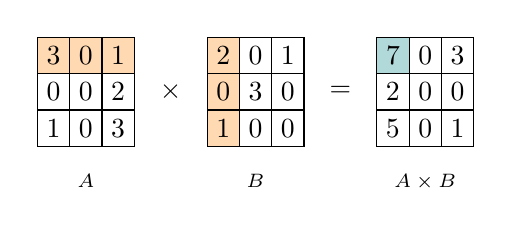
\begin{tikzpicture}[
    2d-arr/.style={matrix of nodes, row sep=-\pgflinewidth, column sep=-\pgflinewidth, nodes={draw}}
  ]

  \matrix (mtr) [2d-arr] {
  %0 & 1 & 1 & |[fill=orange!30]| 1 & |[fill=orange!30]| 0 & |[fill=orange!30]| 0 & 0\\
    |[fill=orange!30]| 3 & |[fill=orange!30]| 0 & |[fill=orange!30]| 1 \\
    0 & 0 & 2 \\
    1 & 0 & 3 \\
  };

  \node[below=of mtr, below=0.3em] {\scriptsize{$A$}};

  %\node[below=of mtr, below=2em] {$1*0 + 1*0 + 1*0 = 6$};

  \node[right=0.2em of mtr] (str) {$ \times $};

  \matrix (K) [2d-arr, right=0.2em of str, nodes={draw}] {
    |[fill=orange!30]| 2 & 0 & 1 \\
    |[fill=orange!30]| 0 & 3 & 0 \\
    |[fill=orange!30]| 1 & 0 & 0 \\
  };
  \node[below=of K, below=0.3em] {\scriptsize{$ B$}};

  \node[right=0.2em of K] (eq) {$=$};

  \matrix (ret) [2d-arr, right=0.2em of eq] {
  %1 & 4 & 3 & |[fill=blue!80!black!30]| 4 & 1\\
    |[fill=teal!30]| 7 & 0 & 3 \\
    2 & 0 & 0 \\
    5 & 0 & 1 \\
  };
  \node[below=of ret, below=0.3em] {\scriptsize{$A \times B$}};

  %\draw[dashed, teal] (mtr-1-3.north east) -- (K-1-1.north west);
  %\draw[dashed, teal] (mtr-1-3.south east) -- (K-3-1.south west);

  %\draw[dashed, blue!80!black] (K-1-1.north east) -- (ret-1-1.north west);
  %\draw[dashed, blue!80!black] (K-3-1.south east) -- (ret-1-1.south west);

\end{tikzpicture}
\end{document}